% !TEX program = xelatex
% vim:foldmethod=marker:foldmarker=<<<,>>>
\documentclass[compress]{beamer}

%<<< Preamble
\usepackage[english]{babel}
\usepackage{metalogo}
\usepackage{listings}
\usepackage{fontspec}
\usepackage{amsmath, amssymb}
\usepackage{stackrel}
\usepackage{tikz}
\usepackage{svg}
\usepackage{unicode-math}
\usepackage{subcaption}
\usepackage[theme=nord,charsperline=60,linenumbers]{jlcode}

\usetheme{Nord}

\setmainfont{Roboto}
% \setsansfont{DejaVu Serif}
% \setmonofont{CaskaydiaCove Nerd Font Mono}
\setmonofont{JuliaMono}


\makeatletter
\def\verbatim@nolig@list{}
\newcommand\pin{%
\parbox[t]{10pt}{\raisebox{0.2pt}{\usebeamercolor[fg]{mybullet}{$\ast$}}}}
\makeatother

\newcommand{\E}[1]{\ensuremath{E\left\{#1\right\}}}
\newcommand{\norm}[1]{\ensuremath{\lVert#1\rVert}}
\newcommand*{\thead}[1]{\multicolumn{1}{c}{\bfseries #1}}

\newfontfamily\tabulartext[SizeFeatures={Size=6}]{Roboto}


\hypersetup{
    colorlinks=true,
    urlcolor=NordBlue
}

\DeclareMathOperator*{\argmax}{argmax}
\DeclareMathOperator*{\Var}{Var}

\AtBeginDocument{
    \fontsize{8}{12}
    \selectfont

}

\AtBeginSection[]
{
    \begin{frame}[c,noframenumbering,plain]
        \tableofcontents[sectionstyle=show/hide,subsectionstyle=show/show/hide]
    \end{frame}
}


\AtBeginSubsection[]
{
    \begin{frame}[c,noframenumbering,plain]
        \tableofcontents[sectionstyle=show/hide,subsectionstyle=show/shaded/hide]
    \end{frame}
}
%>>>

\title{Project I: Apertures}
\subtitle{}
\author{\Large Simon Andreas Bjørn}
\date{\large March 8, 2023}

\begin{document}

\begin{frame}[plain,noframenumbering]
    \maketitle
\end{frame}

\begin{frame} % <<< Unfocused ASA Simulation
    \frametitle{Unfocused ASA Simulation}
    We want to run the \texttt{ASA.m} and inspect the results.
    Running the \texttt{ASA.m} code yields the following to plots
    \begin{columns}
        \begin{column}{0.5\textwidth}
            \begin{figure}
                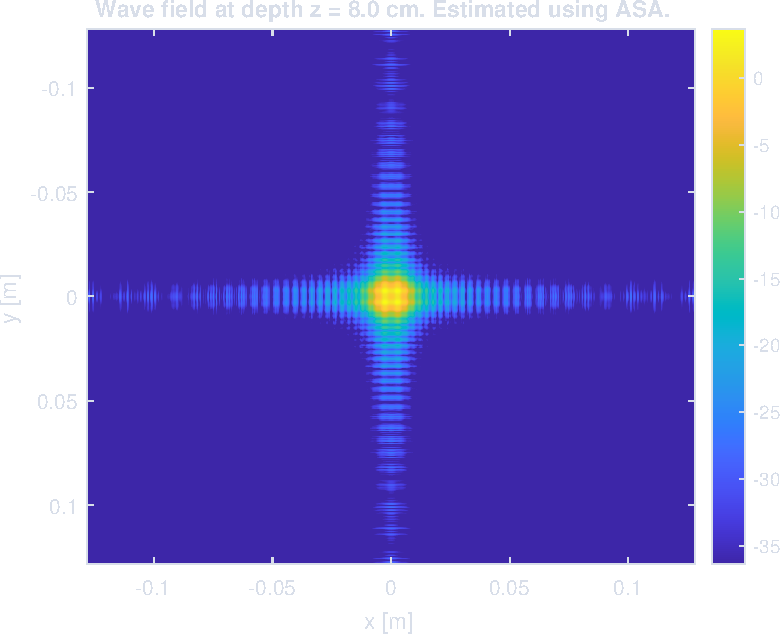
\includegraphics[height=0.5\textheight]{"../1a.pdf"}
            \end{figure}
        \end{column}
        \begin{column}{0.5\textwidth}
            \begin{figure}
                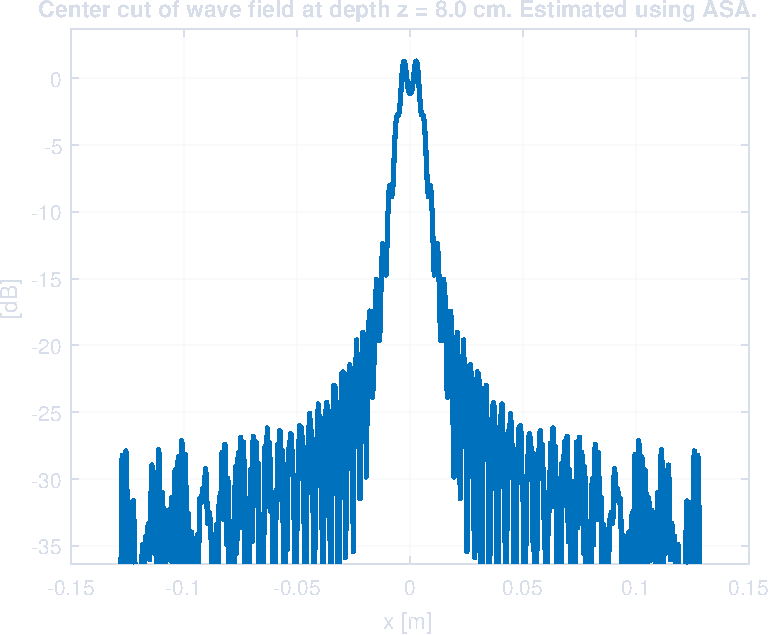
\includegraphics[height=0.5\textheight]{"../1b.pdf"}
            \end{figure}
        \end{column}
    \end{columns}
    \begin{itemize}
        \item Left plot is the wave field $U(x,y,z=z_0)$, of a uniform square point source with $D=15\lambda$
        \item Right plot is the pressure along the x-axis at $y = 0, z=z_0$.
        \item FFT of the Box-function is the sinc.
        \item Square-array = 2d-box function, so its a sinc along x- and y-axis
    \end{itemize}
    The wave field has propagated a minimal amount from the true source at $z=0$.
\end{frame} % >>>

\begin{frame}[fragile] % <<< Unfocused ASA Simulation 2
    \frametitle{Unfocused ASA Simulation 2}
    We want to taper the propagator, and propagate the wave field for some distance $z=0.4$.
    Modifying the \texttt{ASA.m} script with the additions written in the assignment text,
    \begin{columns}
        \begin{column}{0.5\textwidth}
            \begin{figure}
                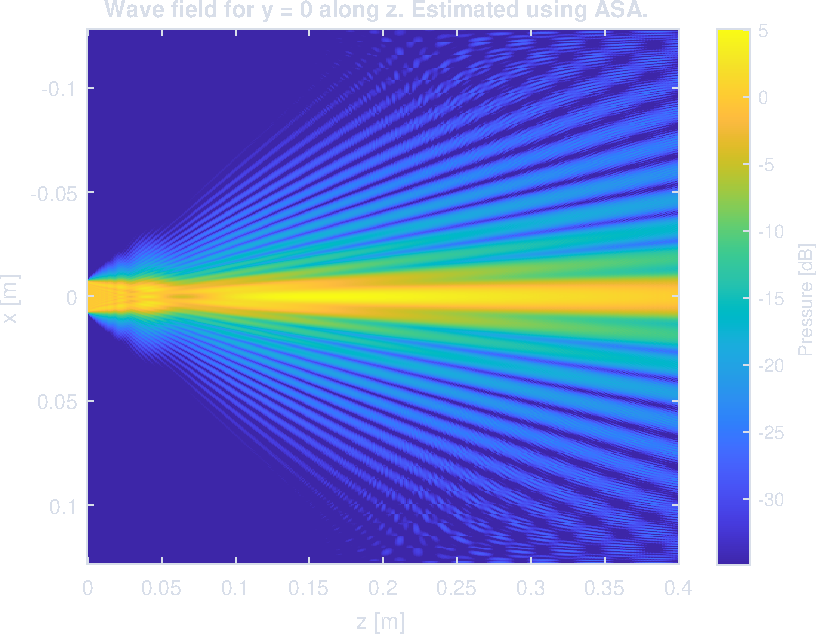
\includegraphics[width=\columnwidth]{"../2a.pdf"}
            \end{figure}
        \end{column}
        \begin{column}{0.5\textwidth}
            \begin{figure}
                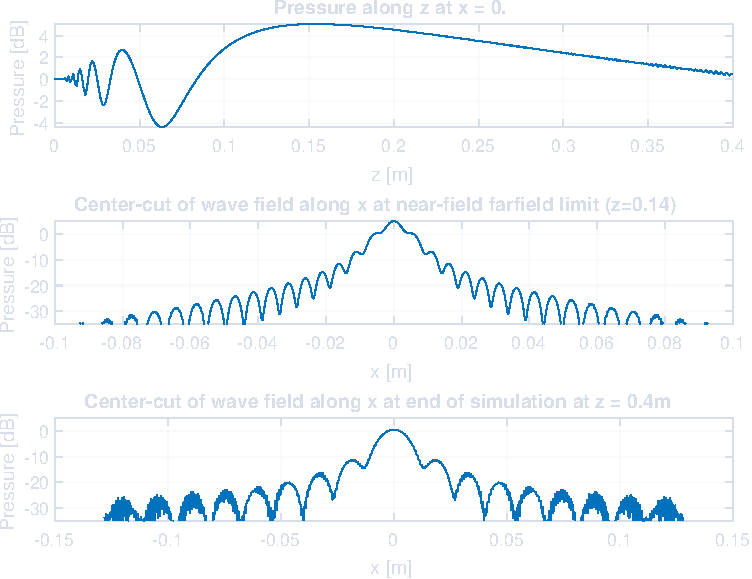
\includegraphics[width=\columnwidth]{"../2b.pdf"}
            \end{figure}
        \end{column}
    \end{columns}
    \vspace{1mm}
    For the near field, I read from the preassure along $z$ at $x=0$, and pick
    $d_nf = 0.014m$. We see that the near field farfield limit closely resembles
    that of the farfield.\\
    \pin Tapering has reduced the effects of the sinc appearance from 1.
    
\end{frame}
% >>>

\begin{frame}[fragile] % <<< Array Pattern - Grating lobes
    \frametitle{Array Pattern - Grating lobes}
    Given an array of $M=24$ elements, we want to find the beampattern of the array
    with different spacings of the elements. Here I use the \texttt{beampattern.m} code.
    \begin{columns}
        \begin{column}{0.52\textwidth}
            \begin{jllisting}[gobble=16, language=Matlab]
                DXs = [P.lambda/4   P.lambda/2 ...
                       P.lambda   2*P.lambda];

                ks = linspace(-1,1,N);
                kx = 2*pi/P.lambda*ks;
                weights = ones(M, 1);

                for dx_idx = 1:numel(DXs)
                    dx = DXs(dx_idx);
                    D = M*dx;
                    xpos = linspace(-D/2, D/2, M);
                    
                    W = beampattern(xpos, kx, weights);
                end
            \end{jllisting}
        \end{column}
        \begin{column}{0.5\textwidth}
            \begin{figure}
                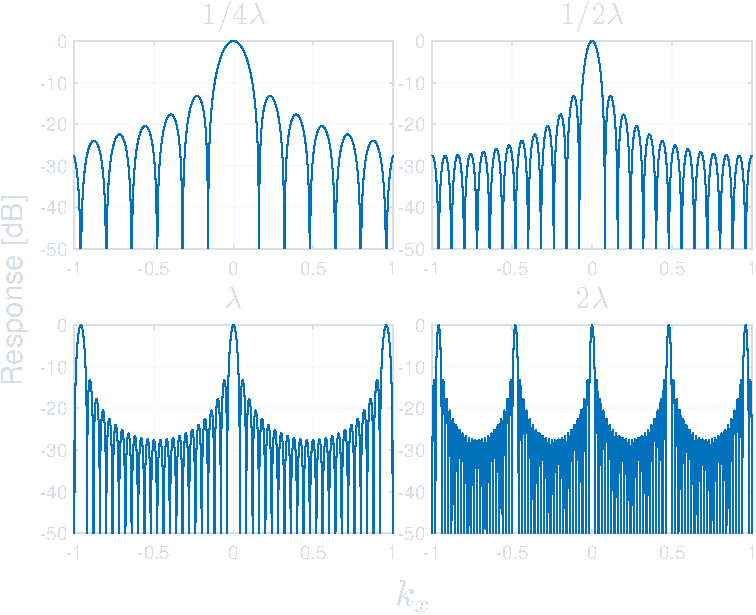
\includegraphics[width=\columnwidth]{"../4.pdf"}
            \end{figure}
        \end{column}
    \end{columns}
    We see that for element distance $D \le \frac{λ}{2}$ we don't see any grating lobes,
    while for $D \ge \frac{λ}{2}$ we see the grating lobes appear at the end of the array
    pattern.
\end{frame}
% >>% >>>

\begin{frame}[fragile] % <<< Element weighting and spacing
    \frametitle{Element weighting and spacing}
    We now want to apply a taper to the array, using a Kaiser windo and see how
    different windows impact the array pattern.
    
    Applying the window is pretty streight forward
    \begin{enumerate}
        \item Create a window of given length and shape
        \item Normalize window so sum of elements are 1
        \item Apply taper to beampattern
    \end{enumerate}

    \begin{jllisting}[gobble=8,language=Matlab]
        beta = betas(beta_idx);
        win = kaiser(M, beta);
        norm_win = win / sum(win(:));
        W = beampattern(xpos, kx, norm_win);
    \end{jllisting}
    Using {\texttt analyzeBP.m} we log the mainlobe width at -3dB and -6dB, as
    well as the max height of the sidelobes.
\end{frame}
% >>>

\begin{frame}[fragile] % <<< Element weighting and spacing 2
    \frametitle{Element weighting and spacing 2}
    We also want to find the white noise gain of the array.
    Since we use a normalized kaiser window, we assume that
    $W^Ha\left(\omega,\tau\right) = 1$ which gives the gain
    $ GW\left(\theta\right)=\norm{\vec{w}}^{-2} $. Plotting the results from
    our logged values we have the following
    \begin{jllisting}[gobble=8,language=Matlab]
        win = kaiser(M, beta); norm_win = win / sum(win(:));
        W = beampattern(xpos, kx, norm_win);
        analyze = analyzeBP(ks, W); GW = 1 / norm(norm_win)^2;
    \end{jllisting}
    \begin{columns}
        \begin{column}{0.5\textwidth}
            \begin{figure}
                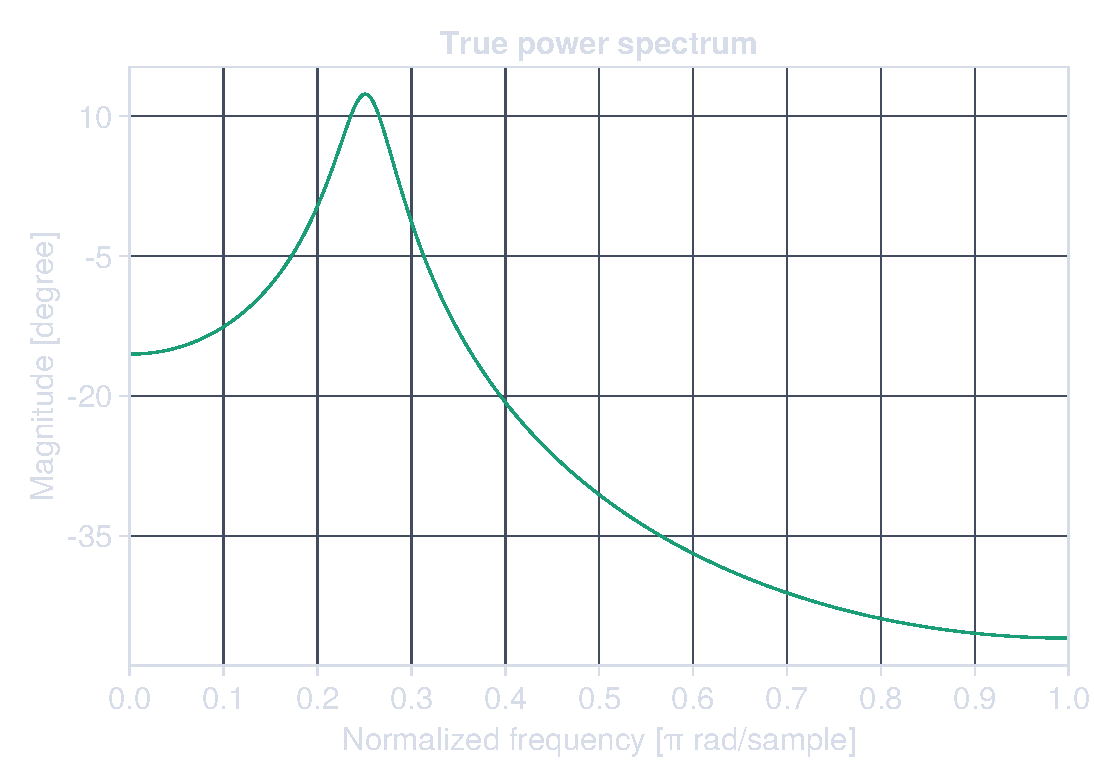
\includegraphics[width=\columnwidth]{"../5.pdf"}
            \end{figure}
        \end{column}
        \begin{column}{0.5\textwidth}
            Looking at the plot to the left, we see that increasing beta
            \begin{itemize}
                \item Increases width of mainlobe
                \item Suppresses the height of the sidelobes
                \item Decreases the white noise gain
            \end{itemize}
            {\bf Conclusion}: there is a trade-off when using the taper. It supresses the 
            sidelobes to some degree at the cost of angular resolution.
        \end{column}
    \end{columns}
\end{frame}
% >>>

\begin{frame} % <<< Irregular Linear Array
    \frametitle{Irregular Linear Array}
    Now we have a irregular linear array with unity weights which we compare to
    the previous.\footnote{\tiny Matlab code from the assignment is used to generate 
    the element positions.}
    \begin{columns}
        \begin{column}{0.5\textwidth}
            \begin{itemize}
                \item Plotting the array pattern gives the plot on the left
                \item Lower maximum sidelobe than ULA with same spacing
                \item Aperture width is 0.3mm smaller than the ULA
                \item With the current spacing corresponding to $d=\frac{1}{2}\lambda$,
                    we see no grating lobes in either array.
            \end{itemize}
        \end{column}
        \begin{column}{0.5\textwidth}
            \begin{figure}
                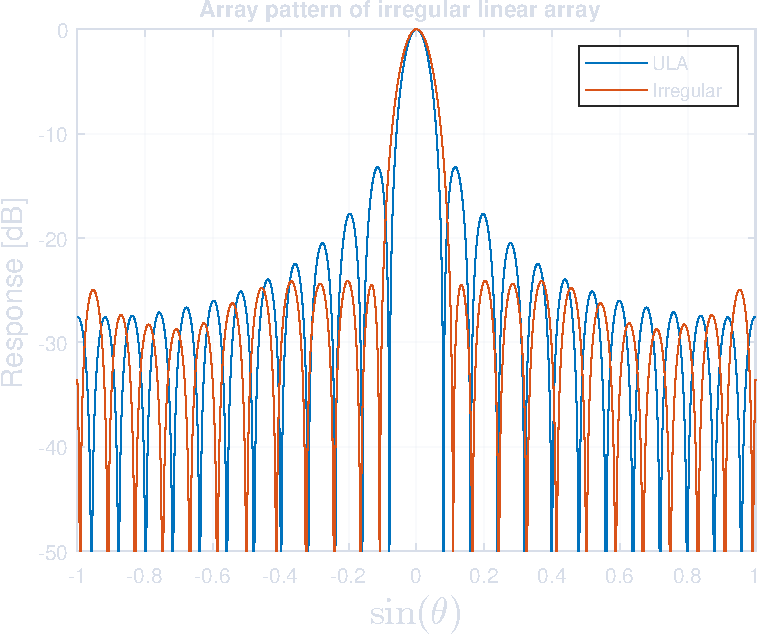
\includegraphics[width=\columnwidth]{"../6a.pdf"}
            \end{figure}
        \end{column}
    \end{columns}
\end{frame} % >>>

\begin{frame} % <<< Irregular Linear Array 2
    \frametitle{Irregular Linear Array 2}
    Comparing the new irregular array to ULA with respect to the beampattern:
    \begin{table}[]
        \tiny
        \begin{tabular}{r|c|c|c|c}
          & -3dB Width {[}k{]} & -6dB Width {[}k{]} & Sidelobe height {[}dB{]} & White Noise Gain \\ \hline
            ULA       & 0.070              & 0.096              & -13.211                  & 24   \\ \hline
            Irregular & 0.086              & 0.117              & -24.111                  & 24              
        \end{tabular}
    \end{table}
    From the table above, we see that 
    \begin{itemize}
        \item The mainlobe is a bit wider while its
        \item Sidelobes are lower. 
        \item Both arrays have similar white noise gain.
    \end{itemize}
    Since both arrays use normalized unit weights, we have that the white noise
    gain is 
    \begin{equation*}
        GW = \norm{\vec{w}}^{-2} = \frac{1}{\left(\sqrt{\sum^{M}{\left(\frac{1}{M}\right)^2}}\right)^2}
        = \frac{1}{M\cdot \frac{1}{M^2}} = M
    \end{equation*}
    where $M$ is the number of elements. Thus, the measured white noise gain is
    as expected, as we have $M=24$ elements.
\end{frame} % >>>

\begin{frame}[fragile] % <<< Steering Irregular Array
    \frametitle{Steering Irregular Array}
    Now we want to apply steering to the irregular array and compare it to the
    ULA.
    
    We want to get find the beampattern of the array with steering, which we apply
    by $W = \left(k_x - k_x^\circ\right)$.
    \begin{columns}
        \begin{column}{0.5\textwidth}
            \begin{figure}
                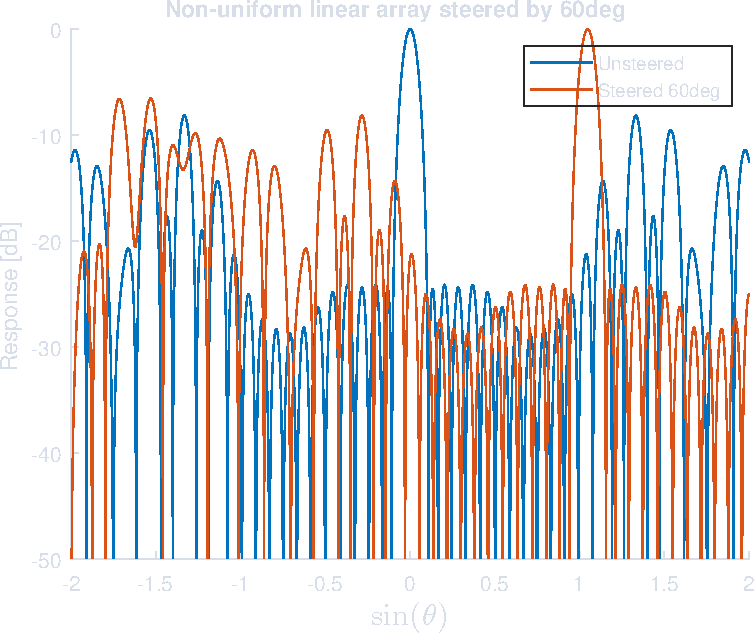
\includegraphics[width=0.8\columnwidth]{"../7a.pdf"}
            \end{figure}
            \begin{jllisting}[gobble=16,language=Matlab]
                ks = linspace(-2, 2, N);
                kx = 2*pi/P.lambda*ks; k0 = pi/(3*d);
                W1 = beampattern(ElPos, kx - k0, norm_win);
            \end{jllisting} 
        \end{column}
        \begin{column}{0.5\textwidth}
            \pin From the plot on the left, we can see the effect of steering
            the array by 60 degrees. However, compared to steering the ULA, we
            see that no grating lobes appear.
            \begin{figure}
                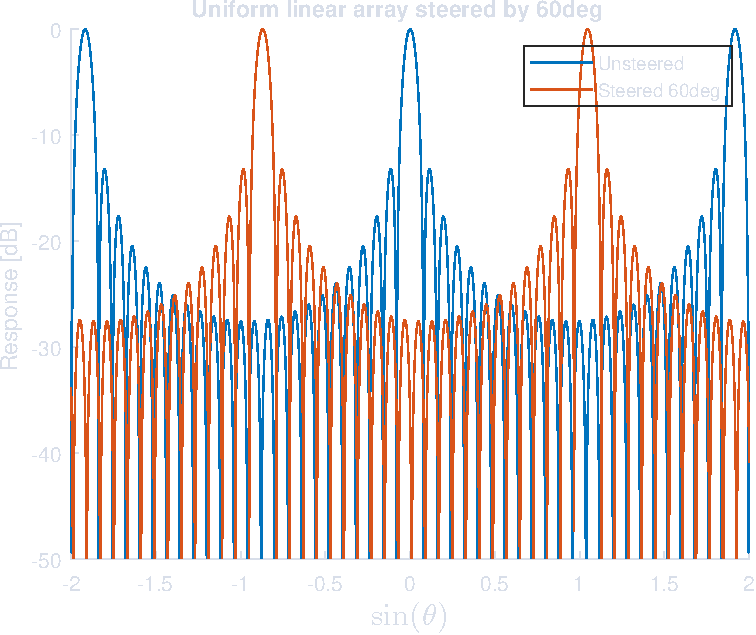
\includegraphics[width=0.7\columnwidth]{"../7b.pdf"}
            \end{figure}
        \end{column}
    \end{columns}
\end{frame} 
% >>>

\begin{frame} % <<< Steering Irregular Array 2
    \frametitle{Steering Irregular Array 2}
    We now want to steer the array different amounts and log the width of the
    mainlobe as a function of the steering angle.

    \begin{columns}
        \begin{column}{0.5\textwidth}
            \begin{figure}
                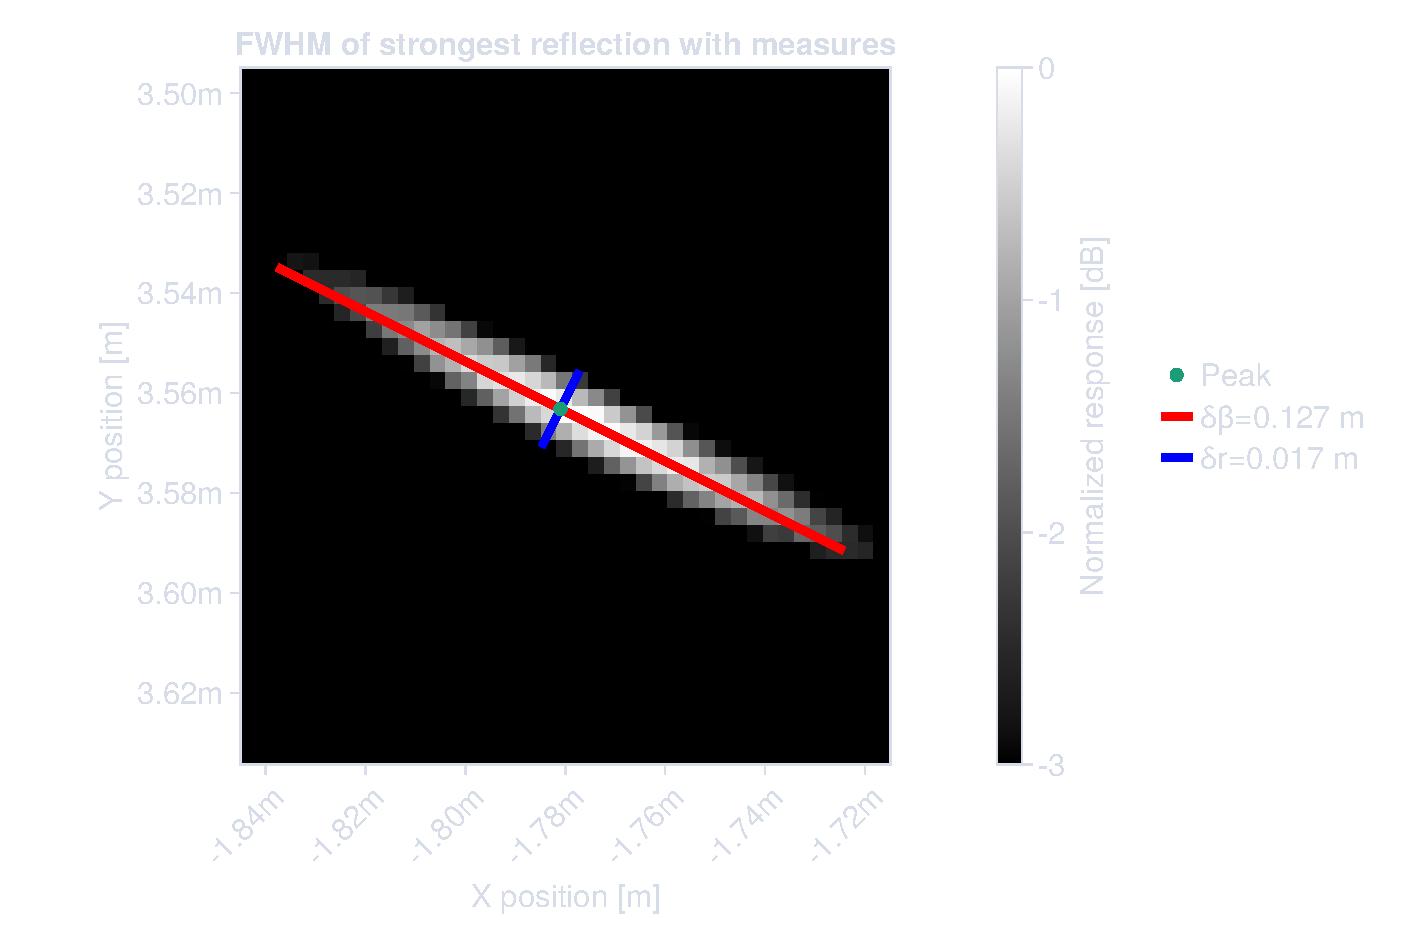
\includegraphics[width=\columnwidth]{"../8.pdf"}
            \end{figure}
        \end{column}
        \begin{column}{0.5\textwidth}
            \begin{itemize}
                \item -3dB and -6dB follows the same shape
                \item Increasing the steering angle widen the main lobe
            \end{itemize}
        \end{column}
    \end{columns}
\end{frame} % >>>

\begin{frame} % <<< Array thinning
    \frametitle{Array thinning}
    We assume an array with $M=101$ elements with spacing $d=\frac{\lambda}{2}$
    We want to analyse the array pattern when a selection of random elements are
    responsive.
    \begin{table}[]
        \tabulartext
        \begin{tabular}{r|l|l|c|c}
                   & -3dB Width    & -6dB Width    & Mean Sidelobe & Max Sidelobe \\ \hline
            25 random elements & 0.0148±0.0017 & 0.0214±0.0026 & -7.5813       & 0.9823       \\ \hline
            50 random elements & 0.0149±0.0016 & 0.0219±0.0013 & -11.4279      & 1.2940       \\ \hline
            75 random elements & 0.0147±0.0015 & 0.0220±0.0002 & -13.1505      & 1.4858       \\ \hline
            Dense array (101)  & 0.0140        & 0.0220        & -13.3277      & - N/A -      \\ \hline
            Minimum Beamwidth  & 0.0180        & 0.0260        & -12.0399      & - N/A -      \\ \hline
            Minimum Sidelobe   & 0.0180        & 0.0260        & -12.0399      & - N/A -     
        \end{tabular}
    \end{table}
    \begin{itemize}
        \item Increasing number of elements narrows mainlobe width
        \item Increasing number of elements suppress sidelobe levels
        \item Dense array performs the best of all arrays analyzed
        \item Both optimized arrays perform identically (code bug)
        \item The optimized arrays supress sidelobes to the etter than 50 elements
    \end{itemize}
\end{frame} 
% >>>

\begin{frame}[fragile] % <<< Element directivity
    \frametitle{Element directivity}
    We want to again consider the regular array from before, with $d=\lambda$ and
    $d=2\lambda$, but this time assume element has finite width $d$.

    We use the formula for the combined array pattern
    \begin{equation*}
        W_{tot}\left(\vec{k}\right) = W_a\left(\vec{k}\right)\cdot W_e\left(\vec{k}\right)
    \end{equation*}
    where $W_e$ is the element response given by
    $W_e\left(\vec{k}\right) = \frac{\sin\left(dk/2\right)}{k/2}$.
    \begin{columns}
        \begin{column}{0.5\textwidth}
            \begin{figure}
                \includegraphics[width=\columnwidth]{"../11.pdf"}
            \end{figure}
        \end{column}
        \begin{column}{0.5\textwidth}
            \begin{itemize}
                \item Grating lobes appear at same places as with array with points
                \item Grating lobes are suppressed when using finite element sizes
            \end{itemize}
            \begin{jllisting}[gobble=16,language=Matlab]
                We = sin(kx*d/2) ./ (kx / 2);
                Wa = beampattern(xpos, kx, weights);
                Wtot = We.'.*Wa;
            \end{jllisting}
        \end{column}
    \end{columns}
\end{frame}
% >>>

\begin{frame}[fragile] % <<< Element directivity 2
    \frametitle{Element directivity but with a twist} 
    Now we want to implement steering to the array.

    We apply steering to the elements and the array the same way as previously
    \begin{columns}
        \begin{column}{0.5\textwidth}
            \begin{figure}
                \includegraphics[width=\columnwidth]{"../12.pdf"}
            \end{figure}
        \end{column}
        \begin{column}{0.52\textwidth}
            \begin{itemize}
                \item For $d=\lambda$ a small skew is observed in the first
                    grating lobes.
                \item The wrapped grating lobes are smaller than for a similar
                    array with point sensors.
            \end{itemize}
            \begin{jllisting}[gobble=16,language=Matlab]
                We = sin((kx-k0)*d/2) ./ ((kx-k0) / 2);
                Wa = beampattern(xpos, kx-k0, weights);
                Wtot = We.'.*Wa;
            \end{jllisting}
        \end{column}
    \end{columns}
\end{frame}
% >>>

\end{document}
